\subsection{UC8 - Visualizzazione dettagli ordinazione}\label{usecase:8}
\begin{figure}[H]
    \centering
    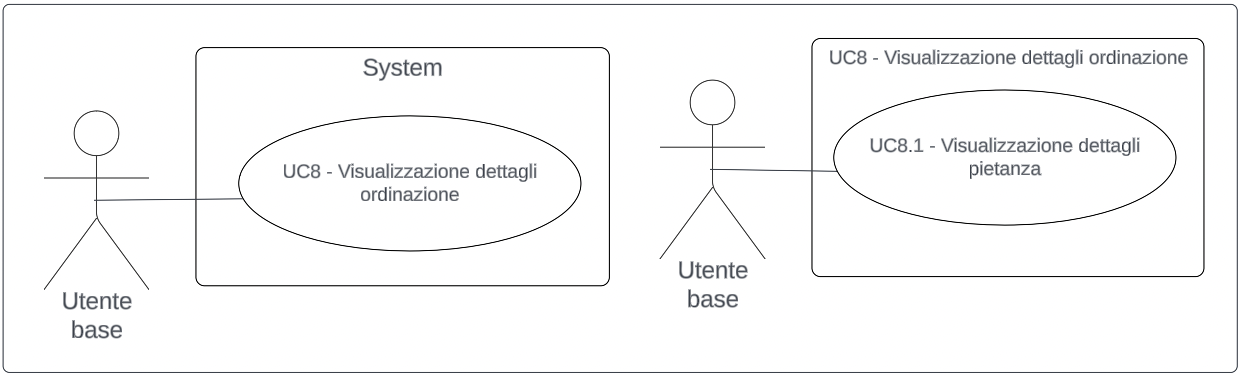
\includegraphics[width=0.9\linewidth]{ucd/ucd8_new.png}
    \caption{Visualizzazione dettagli ordinazione}
\end{figure}
\textbf{Attori}:
\begin{itemize}
    \item Utente base.
\end{itemize}
\textbf{Precondizioni}:
\begin{itemize}
    \item L'utente è connesso al $\textit{Sistema}_G$;
    \item L'utente ha effettuato un $\textit{ordinazione}_G$ (\nameref{usecase:3}).
\end{itemize}
\textbf{Postcondizioni}:
\begin{itemize}
    \item L'utente visualizza il riepilogo dell'ordine includendo anche le pietanze scelte dagli altri utenti.
\end{itemize}
\textbf{Scenario principale}:
\begin{enumerate}
    \item L'utente visualizza la lista di tutte le pietanze ordinate dai partecipanti al tavolo;
    \item Ogni riga della lista presenta i dettagli della pietanza ordinata (\nameref{usecase:8_1}).
\end{enumerate}
\subsubsection{UC8.1 - Visualizzazione dettagli pietanza}\label{usecase:8_1}
\textbf{Attori}:
\begin{itemize}
    \item Utente base.
\end{itemize}
\textbf{Precondizioni}:
\begin{itemize}
    \item L'utente è connesso al $\textit{Sistema}_G$;
    \item L'utente ha effettuato un $\textit{ordinazione}_G$ (\nameref{usecase:3});
    \item L'utente sta visualizzando la lista delle pietanze ordinate.
\end{itemize}
\textbf{Postcondizioni}:
\begin{itemize}
    \item L'utente visualizza i dettagli della pietanza ordinata.
\end{itemize}
\textbf{Scenario principale}:
\begin{enumerate}
    \item L'utente visualizza i dettagli della pietanza ordinata, ovvero:
    \begin{enumerate}
        \item Nome del pasto ordinato;
        \item Quantità ordinata;
        \item La persona che ha effettuato l'ordine.
    \end{enumerate}
\end{enumerate}
\newpage